\documentclass [11pt, a4wide, twoside]{article}

\usepackage{times}
%\usepackage{epsfig}
\usepackage{ifthen}
\usepackage{xspace}
\usepackage{fancyhdr}
\usepackage{graphicx}
\usepackage[colorlinks,urlcolor=blue]{hyperref}
\newcommand{\yellowbox}[1]{\fcolorbox{yellow}{yellow}{\bfseries\sffamily\scriptsize#1}}
\newcommand{\nb}[2]{{\yellowbox{#1}\yellowbox{#2}}}

\newcommand\todo[1]{\nb{TO DO}{#1}}

% solution switch
\newboolean{showsolution}
\setboolean{showsolution}{true} 
\setboolean{showsolution}{false}


%layout
\topmargin      -5.0mm
\oddsidemargin  6.0mm
\evensidemargin -6.0mm
\textheight 215.5mm
\textwidth      160.0mm
\parindent        1.0em
\headsep          10.3mm
\headheight        12pt
\lineskip    1pt
\normallineskip     1pt

%header
\lhead{Programming Languages \\ 2021}

\rhead{Prof. O. Nierstrasz\\
Mohammadreza Hazhirpasand, Joel Niklaus}
\lfoot{page \thepage}
\rfoot{\today}
\cfoot{}

\renewcommand{\headrulewidth}{0.1pt}
\renewcommand{\footrulewidth}{0.1pt}

\renewcommand{\thesubsection}{\arabic{subsection}}

%enumeration
\newenvironment{myitemize}{%
     \begin{itemize}
     \setlength{\itemsep}{0cm}}
     {\end{itemize}}

\newenvironment{myenumerate}{%
     \begin{enumerate} \setlength{\itemsep}{0cm}}
     {\end{enumerate}}


%solution
\ifthenelse{\boolean{showsolution}}
   {  \newcommand{\solution}[1]{
   	\noindent\underline{\textbf{Answer:}}\\[2mm]
   	 \textsl{#1}
	 \vspace{10pt}
	 \normalsize
	}
  }
  {  \newcommand{\solution}[1]{} }

\newcounter{exnum}
\def\xexercise{\fontsize{12}{10}\fontseries{bx}\selectfont}
\def\xnormal{\fontseries{m}\fontshape{n}\selectfont}


\newcommand{\exercise}[1]{%
     {\addtocounter{exnum}{1}\vskip 0.8cm{\xexercise \noindent Exercise
\arabic{exnum} (#1)} \xnormal} \vskip 0.3cm} 
 \newcommand{\aufgabe}[1]{
     {\addtocounter{exnum}{1}\vskip 0.8cm{\xexercise \noindent Aufgabe
\arabic{exnum} (#1)} \xnormal} \vskip 0.3cm} 

\pagestyle{fancy}


% ===============ABBREVIATIONS==============================
\newcommand{\eg}{\emph{e.g.,}\xspace}
\newcommand{\ie}{\emph{i.e.,}\xspace}
\newcommand{\etc}{\emph{etc.}\xspace}


\begin{document}

% title
\section*{\ifthenelse{\boolean{showsolution}}{Solution }{}\xspace{}Exam Programming Languages}
\rule{\textwidth}{1pt}\\[1mm]
Date: Friday, 03.06.2016.\\
Duration: 70 minutes\\
Material: You are NOT allowed to use any material (e.g., script, exercises including solutions, notes, electronic devices...)\\
Number of exercises: 6\\
Total points: 80 \\
\rule{\textwidth}{1pt}\\[5mm]
Firstname, lastname: \rule{200pt}{0.5pt}\\[5mm]
Matrikel: \rule{200pt}{0.5pt}\\[5mm]
Put your name on each extra page you deliver.\\
Consecutively number all pages. Total number of extra pages: \rule{45pt}{0.5pt}\\
\rule{\textwidth}{1pt}

\newpage
% - - - - - - - - - - - - - - - - - - - - - - - - - - - - - - - - - - - - - - - - - - - - - - - - - - - - - - - - - - - - - - - - - - -

\exercise{20 Points}
\noindent
%
Answer the following questions (do not write more than 3 sentences):

\begin{myenumerate}

\item What is a tail-recursive function and what is the advantage compared to a non-tail-recursive function?
\solution{Tail-recursive means calling itself is the last thing the function does. Advantage is reusing the stack.}\vspace{3cm}

\item  What is a higher-order function? Give an example.
\solution{A function that takes another function as an argument or returns a function. example: map}\vspace{3cm}

\item What is the difference between a static and a dynamic type? Give an example.
\solution{The static type of a variable or expression is a type which can be determined by the type inference  system solely based on the program code, thus in at compile time. In contrast, the dynamic type of a variable cannot be determined in such a way because the variable may take on different values at runtime. Example:\\
Object x = new Vector();\\
the static type of x is Object, the dynamic type is Vector().}\vspace{3cm}

\item What are the operations one can perform in lambda calculus? 
\solution{alpha conversion, betta reduction, eta reduction}\vspace{3cm}

\item What is a fixed point of a function? 
\solution{A fixed point of a function f is a value p such that f p = p.}\vspace{3cm}

\newpage
\item What is the difference between syntax and semantics? 
\solution{Syntax: the arrangement of words and phrases to create well-formed sentences in a language \\
Semantics: the meaning of a word, phrase, sentence or text\\
You can create well-formed sentences (according to the syntax) that don't have a meaning (according to semantics).} \vspace{3cm}

\item  What is the Principle of Substitutability?
\solution{An instance of a subtype can always be
used in any context in which an instance
of a supertype was expected} \vspace{3cm}

% \item \todo{JS/prolog QUESTION}Explain how it is possible to use the concept of recursion in the $\lambda$-calculus, despite the above fact. 
% \solution{We know by the Fixed-Point theorem that every $\lambda$-expression $e$ has a fixed point $p$, i.e. $(e ~p) \equiv p$. Thus recursive functions (i.e. recursive $\lambda$-expressions) can be expressed as fixed-points of other suitable expressions, which must be well-defined. Finding this fixed-point is achieved in the (untyped) lambda-calculus by means of a fixed-point combinator called the \emph{Y-combinator}. So if we define a function $p$ to be the Y-combinator applied to an expression $e$, the result of this application is the again the expression with the desired function as argument, $e~p$, which equals $p$.} \vspace{3cm}


% \item How does contravariance support subtyping?
% \solution{Because the contravariance parameter type will always end in the correct result subclass since $f_y$ is a superset of $f_x$} \vspace{3cm}


% \item How does contravariance support subtyping?\textbf{( 1 Point )}
% \solution{Because the contravariance parameter type will always end in the correct result subclass since $f_y$ is a superset of $f_x$} \vspace{3cm}

\item How does Java supports subtyping? How does it support specializations?

\solution{\emph{subtyping}: Interfaces \& inheritance, \emph{specialization}: Inheritance.} \vspace{3cm}

\item Where do you in Javascript define properties that are shared between a group of objects (i.e., static members in Java)?\
\solution{Either using the same prototype and defining on the prototype side or in a global scope.}\vspace{3cm}

\item How would you define a logical negation operator \texttt{neg(X)} in Prolog?
\solution{\texttt{neg(X) :- X, !, fail. neg(\_).}} \vspace{3cm}

\end{myenumerate}


\newpage
% - - - - - - - - - - - - - - - - - - - - - - - - - - - - - - - - - - - - - - - - - - - - - - - - - - - - - - - - - - - - - - - - - - -

\exercise{6 Points}
\noindent
%

A very junior programmer wanted to write the ``hello world'' program in Postscript. Here is the result: 

\begin{small}
\begin{verbatim}
    /Times-Roman findfont
    18 scalefont
    setfont
    100 500 moveto

    /myprint {
        exch
        /mystring exch def
        show mystring show
    } def

    /mystring (Hello) def
    mystring
    /mystring (World) def
    mystring
    myprint
    showpage
\end{verbatim}
\end{small}

\begin{myenumerate}
\item Did the programmer succeed? If not explain what the output is and why. How can the program can be fixed to achieve the junior programmer goal?
\end{myenumerate}

\solution{The result is WorldHello since /myprint swaps on the stack, redefines mystring as Hello (destroying it on the stack) and shows World then shows mystring.\\
better:\\
(Hello World) show\\
}



\newpage
% - - - - - - - - - - - - - - - - - - - - - - - - - - - - - - - - - - - - - - - - - - - - - - - - - - - - - - - - - - - - - - - - - - -

\exercise{18 Points}
\noindent
%

\begin{figure}[htb]
\begin{minipage}{.65\textwidth}
A \emph{triangular number} is the number of objects that can be arranged in a triangle as is shown in Fig. 1. This is how bowling pins, pool balls, or snooker balls are arranged. The figure shows the first six triangular numbers: 1, 3, 6, 10, 15, 21.

The \emph{tetrahedral number} represents the number of objects arranged in a pyramid (more precisely, a tetrahedron) built up from triangles as shown in the Figure.
\end{minipage}
\begin{minipage}[c]{.35\textwidth}
    \center{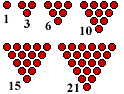
\includegraphics[width=3cm]{images/triang}\caption{Triangular numbers.\label{figure:triangularNumbers}}}
\end{minipage}
\end{figure}

\noindent The exercise:
\begin{myenumerate}
\item Write a function to calculate the n-th triangular number in Haskell.

\vspace{4cm}

\item Write a function to calculate the n-th tetrahedral number in Haskell.

\vspace{4cm}


\item Infer the type of the following function and explain your steps. Is the function monomorphic or polymorphic? 
\begin{small}
\begin{verbatim}
myMap f [] = f
myMap f (x:xs) = myMap (x (f+1)) xs
\end{verbatim}
\end{small}

\end{myenumerate}
\solution{\fontsize{8pt}{10pt}
\begin{verbatim}
triangular 0            = 0
triangular n            = n + triangular (n-1)

tetrahedral 0        = 0
tetrahedral n        = (triangular n) + (tetrahedral (n-1))

myMap :: Num a => a -> [a -> a] -> a  
\end{verbatim}}

\newpage
% - - - - - - - - - - - - - - - - - - - - - - - - - - - - - - - - - - - - - - - - - - - - - - - - - - - - - - - - - - - - - - - - - - -

\exercise{12 Points}
\noindent
%
\begin{enumerate}
\item Consider the following $\lambda$-expressions. Indicate which occurrences of
variables are bound and which ones are free in the expressions.

\begin{enumerate}
\item \texttt{($\lambda$ a b .~c a b) a b ($\lambda$ c d .~d c)($\lambda$ e f .~f) } \vspace{1cm}

\item \texttt{(($\lambda$ u v .~$\lambda$ w .~w ($\lambda$ x .~x(u)) (v)) (y)) ($\lambda$ z .~$\lambda$ y .~z(y))}\vspace{1cm}

\item \texttt{($\lambda$ y .~$\lambda$ x .~z(x($\lambda$ x .~y(z)))) ($\lambda$ z .~y(x(z)))}\vspace{1cm}
\end{enumerate}
\item Reduce the following $\lambda$-expression to its normal form if possible 

\texttt{($\lambda$ x y .~y x) ($\lambda$ x y .~y x)($\lambda$ x .~x x)($\lambda$ y .~y)} 
\end{enumerate}
\solution{\fontsize{9pt}{11pt}\texttt{($\lambda$ a b .~c a b) a b ($\lambda$ c d .~d c)($\lambda$ e f .~f) }\\
\texttt{($\lambda$ a b .~f b b) f f ($\lambda$ c d .~b b)($\lambda$ e f .~b) }\\

\noindent
\texttt{(($\lambda$ u v .~$\lambda$ w .~w ($\lambda$ x .~x(u)) (v)) (y)) ($\lambda$ z .~$\lambda$ y .~z(y))}\\
\texttt{(($\lambda$ u v .~$\lambda$ w .~b ($\lambda$ x .~b(b)) (b)) (f)) ($\lambda$ z .~$\lambda$ y .~b(b))}\\

\noindent
\texttt{($\lambda$ y .~$\lambda$ x .~z(x($\lambda$ x .~y(z)))) ($\lambda$ z .~y(x(z)))}\\
\texttt{($\lambda$ y .~$\lambda$ x .~f(b($\lambda$ x .~b(f)))) ($\lambda$ z .~f(f(b)))}\\\\

\noindent
\texttt{($\lambda$ x y .~y x) ($\lambda$ x y .~y x)($\lambda$ x .~x x)($\lambda$ y .~y)} \\
\texttt{($\lambda$ x .~x x)($\lambda$ x y .~y x)($\lambda$ y .~y)} \\
\texttt{($\lambda$ x y .~y x)($\lambda$ x y .~y x)($\lambda$ y .~y)}\\ 
\texttt{($\lambda$ y .~y)($\lambda$ x y .~y x)} \\
\texttt{($\lambda$ x y .~y x)} \\}


\newpage
% - - - - - - - - - - - - - - - - - - - - - - - - - - - - - - - - - - - - - - - - - - - - - - - - - - - - - - - - - - - - - - - - - - -
\exercise{12 Points}
\noindent Suppose you have a small JavaScript program with a database of people:
\begin{verbatim}
var alice = Object.create(person);
alice.name = "Alice";
alice.age = 22;

var bob = Object.create(person);
bob.name = "Bob";
bob.age = 29;

var cyril = Object.create(person);
cyril.name = "Bob";
cyril.age = 45;
\end{verbatim}


\begin{enumerate}
        \item What is the prototype of Alice, Bob and Cyril?
        \vspace{5cm}
        \solution{\texttt{Person}}

%        \item You realize, you need to change the parent of Alice and Bob to \texttt{Employee}, the Cyril to \texttt{Manager}. How would you do it?
%        \vspace{5cm}
%        \solution{\begin{verbatim}
var employee = Object.create(person);
var manager = Object.create(person);

alice.__proto__ = employee.
bob.__proto__ = employee.
cyril.__proto__ = manager.
\end{verbatim}
}
%
        \item Lets say Cyril is a manager. A manager has to be responsible. How would make Cyril (only Cyril, not Alice and Bob) respond to the message \texttt{isResponsible}?
        \vspace{5cm}
        \solution{\begin{verbatim}
manager.isResponsible = function() {
    alert("I am very responsible");
}
\end{verbatim}
}

\newpage
        \item Bob wants to be manager as well, so he tries to be responsible as well. How would you make Bob to become responsible?
        \vspace{5cm}
        \solution{\begin{verbatim}
bob.isResponsible = manager.isResponsible.
\end{verbatim}
}
\end{enumerate}


\newpage
% - - - - - - - - - - - - - - - - - - - - - - - - - - - - - - - - - - - - - - - - - - - - - - - - - - - - - - - - - - - - - - - - - - -

\exercise{12 Points}

Consider the following directed graph:

\begin{figure}[h]
\centering{\fbox{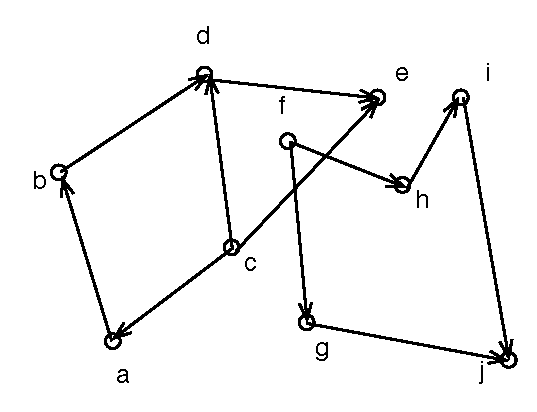
\includegraphics[width=6cm]{images/map.pdf}}}
\end{figure}

Write a Prolog database consisting of the following predicates:

\begin{enumerate}
\renewcommand{\theenumi}{\alph{enumi}}

\item \texttt{line(p1,p2)} that is true iff there is a direct connection from \texttt{p1} to \texttt{p2}.

\item \texttt{triangle(p1,p2,p3)} that is true iff \texttt{p1}, \texttt{p2}, and \texttt{p3} form a triangle (independent of the connection directions).

\item \texttt{quadrangle(p1,p2,p3,p4)} that is true iff \texttt{p1}, \texttt{p2}, \texttt{p3}, and \texttt{p4} form a quadrangle (independent of the connection directions).

\item \texttt{reachable(p1,p2)} that is true iff there is a directed path from \texttt{p1} to \texttt{p2} (i.e. iff \texttt{p2} is reachable from \texttt{p1} respecting the connection directions).
\end{enumerate}

\solution{\begin{verbatim}
connection(A,B) :- line(A,B); line(B,A).
in(X,[X|_]).
in(X,[_|L]):- in(X,L).

line(a,b).
line(b,d).
line(c,a).
line(c,d).
line(c,e).
line(d,e).
line(f,g).
line(f,h).
line(g,j).
line(h,i).
line(i,j).


triangle(A,B,C) :- connection(A,B), connection(B,C), connection(C,A).


quadrangle(A,B,C,D) :- connection(A,B), connection(B,C), connection(C,D), connection(D,A), 
                       not(in(D,[A,B,C])).

reachable(X,Y) :- line(X,Y).
reachable(X,Y) :- line(X,Z), reachable(Z,Y).
\end{verbatim}
}

% - - - - - - - - - - - - - - - - - - - - - - - - - - - - - - - - - - - - - - - - - - - - - - - - - - - - - - - - - - - - - - - - - - -
\newpage
\subsection*{Points}

\begin{minipage}[t]{120pt}
\textbf{Exercise 1}
\vspace{5pt}\\
\begin{tabular}{|c|c|c|c|}
\hline
Task & Points & Score \\\hline
1  & 2 & \\\hline
2  & 2 & \\\hline
3  & 2 & \\\hline
4  & 2 & \\\hline
5  & 2 & \\\hline
6  & 2 & \\\hline
7  & 2 & \\\hline
8  & 2 & \\\hline
9  & 2 & \\\hline
10 & 2 & \\\hline
\textbf{Total} & \textbf{20} &\\\hline\hline
\end{tabular}
\end{minipage}
\begin{minipage}[t]{120pt}


\textbf{Exercise 2}
\vspace{5pt}\\
\begin{tabular}{|c|c|c|c|}
\hline
Task & Points & Score \\\hline
1 & 6 & \\\hline
\textbf{Total} & \textbf{6} &\\\hline\hline
\end{tabular}
\end{minipage}
\begin{minipage}[t]{120pt}


\textbf{Exercise 3}
\vspace{5pt}\\
\begin{tabular}{|c|c|c|c|}
\hline
Task & Points & Score \\\hline
1 & 6 & \\\hline
2 & 6 & \\\hline
2 & 6 & \\\hline
\textbf{Total} & \textbf{18} &\\\hline\hline
\end{tabular}
\end{minipage}
\begin{minipage}[t]{120pt}


\textbf{Exercise 4}
\vspace{5pt}\\
\begin{tabular}{|c|c|c|c|}
\hline
Task & Points & Score \\\hline
1(a) & 2 & \\\hline
1(b) & 2 & \\\hline
1(c) & 2 & \\\hline
2 & 6 & \\\hline
\textbf{Total} & \textbf{12} &\\\hline\hline
\end{tabular}
\end{minipage}

\noindent
\begin{minipage}[t]{120pt}

\vspace{1cm}

\textbf{Exercise 5}
\vspace{5pt}\\
\begin{tabular}{|c|c|c|c|}
\hline
Task & Points & Score \\\hline
1 & 3 & \\\hline
2 & 3 & \\\hline
3 & 3 & \\\hline
4 & 3 & \\\hline
\textbf{Total} & \textbf{12} &\\\hline\hline
\end{tabular}
\end{minipage}
\begin{minipage}[t]{120pt}
\vspace{1cm}

\textbf{Exercise 6}
\vspace{5pt}\\
\begin{tabular}{|c|c|c|c|}
\hline
Task & Points & Score \\\hline
a & 3 & \\\hline
b & 3 & \\\hline
c & 3 & \\\hline
d & 3 & \\\hline
\textbf{Total} & \textbf{12} &\\\hline\hline
\end{tabular}
\end{minipage}
\begin{minipage}[t]{120pt}
\vspace{1cm}

\textbf{TOTAL}
\vspace{5pt}\\
\begin{tabular}{|c|c|c|c|}
\hline
Exercise & Points & Score \\\hline
1 & 20 & \\\hline
2 & 6 & \\\hline
3 & 18 & \\\hline
4 & 12 & \\\hline
5 & 12 & \\\hline
6 & 12 & \\\hline
\textbf{Total} & \textbf{80} &\\\hline\hline
\end{tabular}
\end{minipage}
\end{document}
